\section{Authentication Framework}\label{sec:security-authN}

CFI-Care employs a split authentication strategy tailored to the specific security profiles of web browsers and mobile applications. 
Both flows are alike in the application of \ac{OIDC} and short-lived \acp{JWT}.

\subsection{Web Browser Authentication}

Browser-based authentication is enforced at the edge by the Nginx API Gateway using \texttt{oauth2-proxy} (with the \texttt{auth\_request} module).

\paragraph{Gateway-mediated OIDC Flow}
When an unauthenticated user accesses the dashboard, the gateway redirects the browser to Keycloak via the Authorization Code Flow with PKCE. 
Upon successful authentication, \texttt{oauth2-proxy} establishes a session, issues secure HTTP-only cookies, and injects the \ac{JWT} into the \texttt{Authorization: Bearer} header for all upstream requests to the BFF.

\begin{figure}[H]
    \centering
    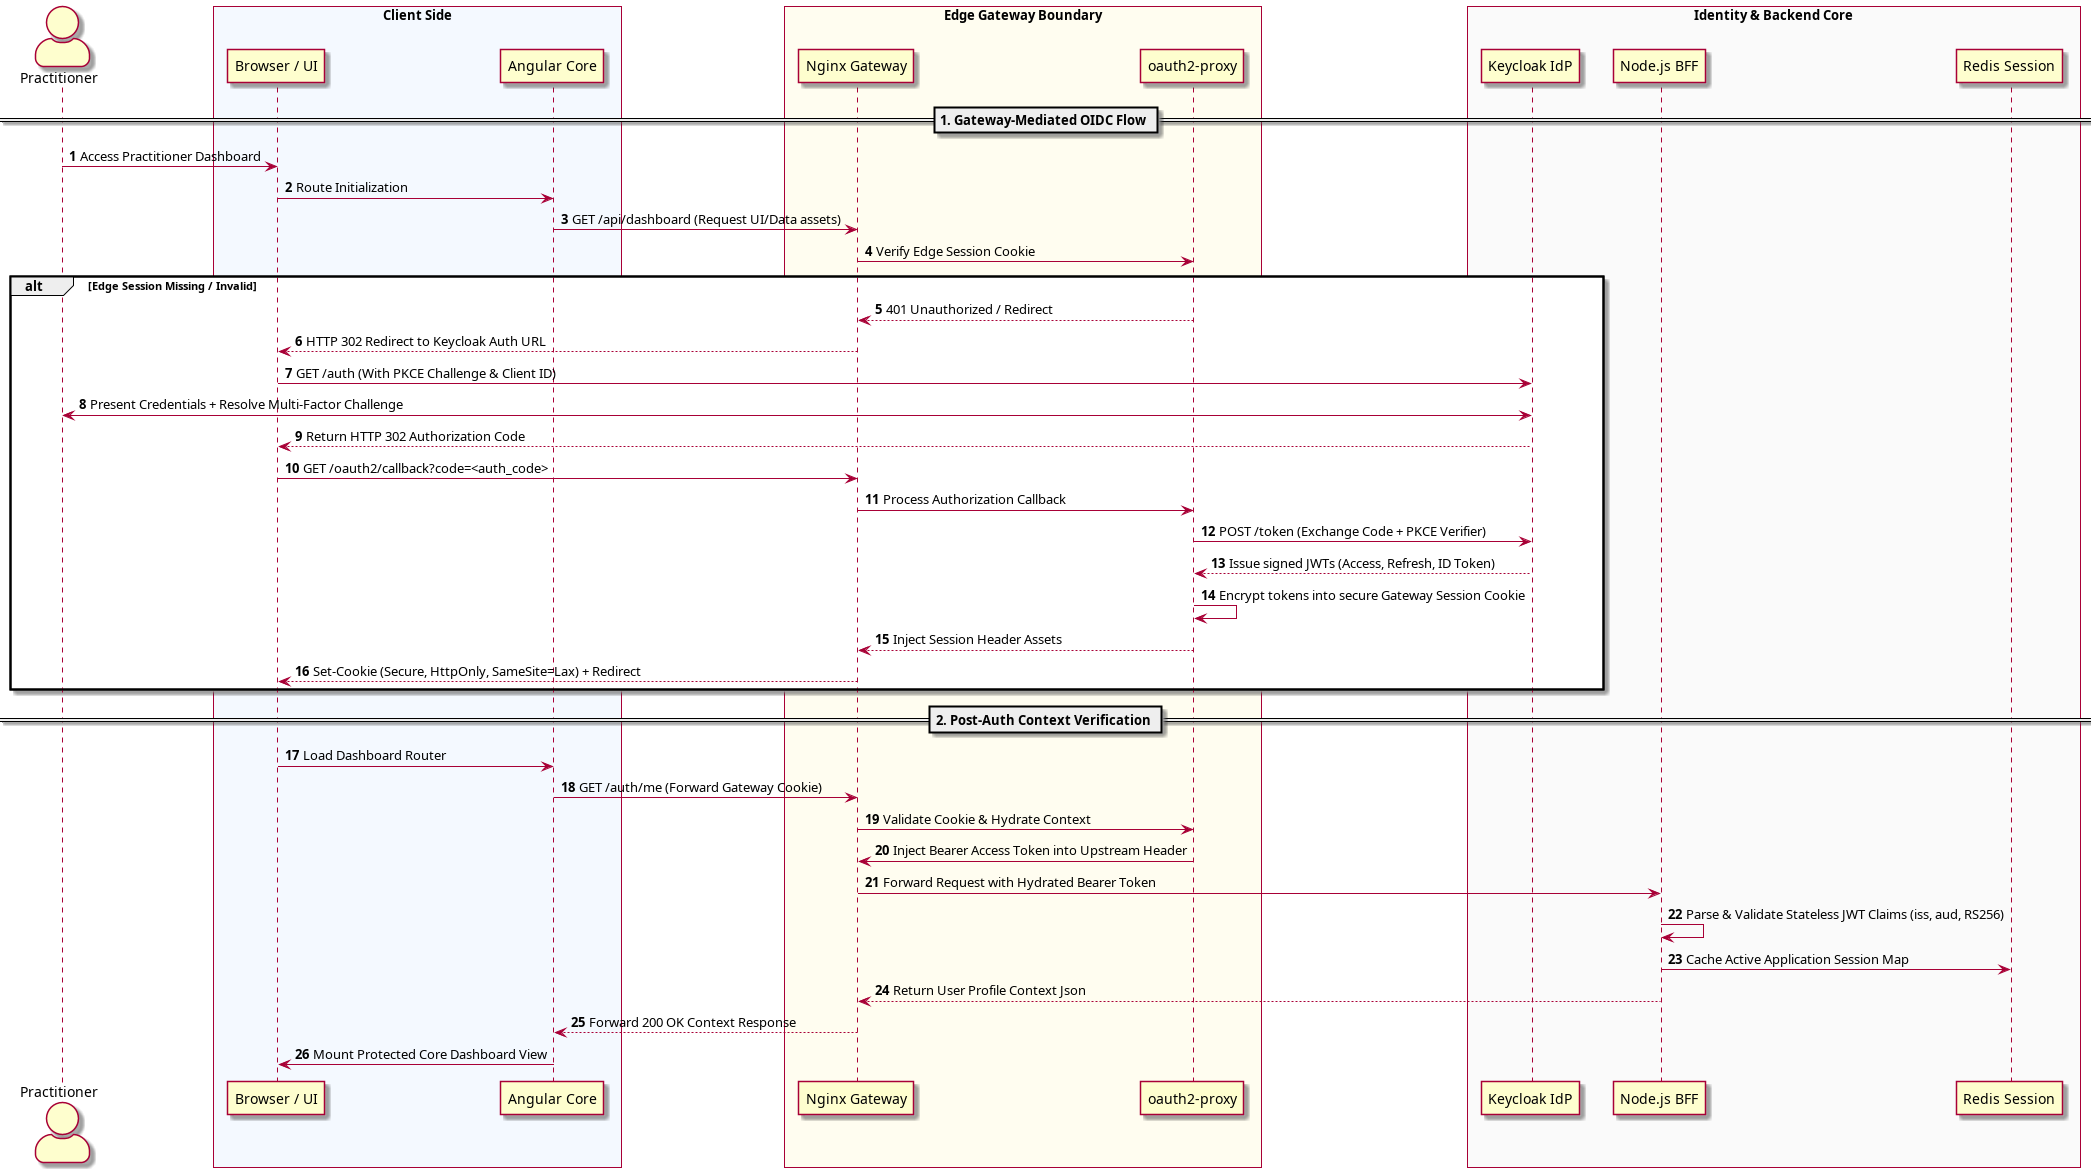
\includegraphics[width=0.9\linewidth]{Security/images/browser-tokens-flow.png}
    \caption{Browser Authentication Sequence: Gateway-mediated OIDC flow and session cookie management.}
    \label{fig:browser-tokens-flow}
\end{figure}

\paragraph{Client-Side Security (Angular)}
The Angular frontend complements the backend security through two primary mechanisms:
\begin{itemize}
    \item \textbf{Route Guards:} Functional guards intercept navigation attempts, verifying authentication status via the BFF's \texttt{/auth/me} endpoint before allowing access to protected views.
    \item \textbf{401 Interceptor:} A global HTTP interceptor monitors outbound requests. If the backend returns a 401 Unauthorized status (e.g due to session expiry), the interceptor clears the local state and redirects the user to the login page.
    \item \textbf{Credential Handling:} All authentication-related requests utilize the \\ \texttt{withCredentials: true} flag to ensure the secure transmission and reception of session cookies.
\end{itemize}

\subsection{Mobile Authentication}

Unlike the browser flow, mobile clients interact directly with the Identity Provider using the \texttt{flutter\_appauth} library.

\paragraph{Mobile Authorization Flow}
The Flutter application implements the Authorization Code Flow with PKCE. 
Once authenticated, tokens are stored in \textbf{Android Keystore}, providing protection against token extraction. 

\begin{figure}[H]
    \centering
    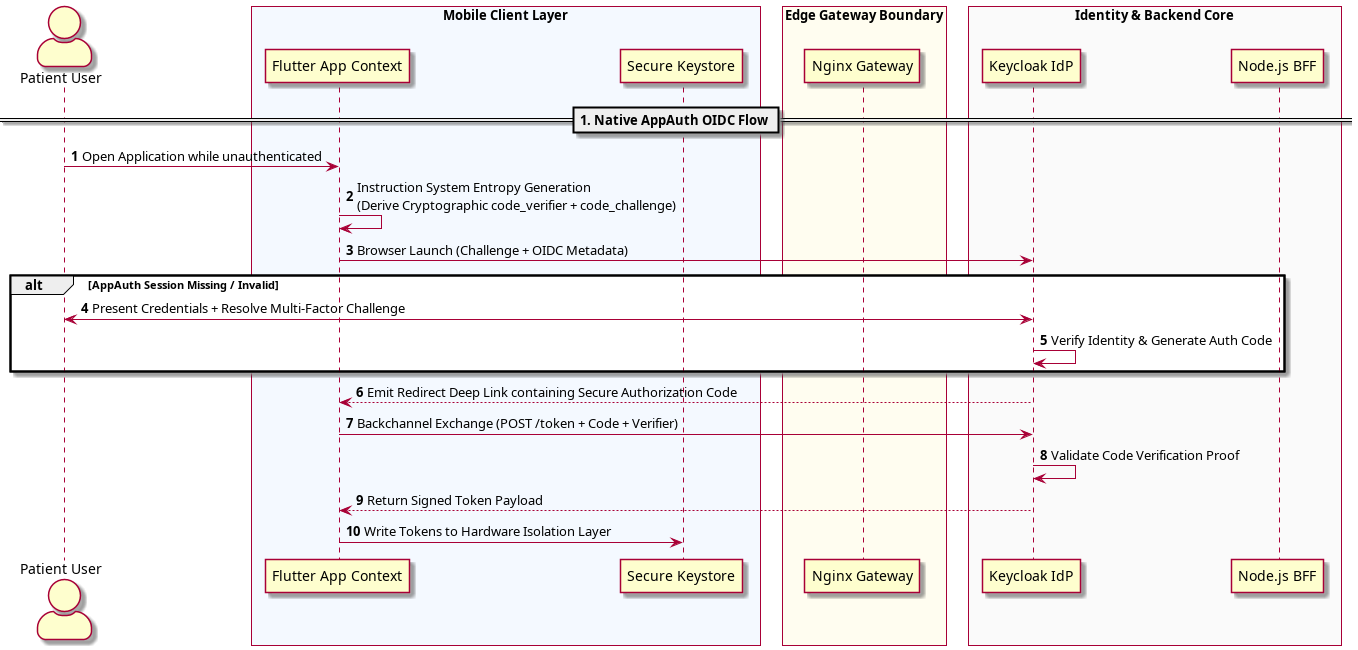
\includegraphics[width=0.8\linewidth]{Security/images/Mobile-tokens-flow.png}
    \caption{Mobile Authentication Flow: Native AppAuth integration and secure token persistence.}
    \label{fig:mobile-tokens-flow}
\end{figure}

\paragraph{Token Refresh Logic}
While the browser flow relies on the gateway for silent refreshes, the mobile app manages its own lifecycle. 
Upon receiving a 401 response, the app attempts a refresh grant,
if successful, the original request is retried; otherwise, the session is invalidated locally.

\subsection{Session Management and Revocation}

To support session tracking and auditing, the BFF utilizes \texttt{express-session} backed by a \textbf{Redis} store.

\paragraph{Session Hardening}
Session cookies are hardened with the following attributes:
\begin{itemize}
    \item \textbf{HttpOnly \& Secure:} Prevents JavaScript access and mandates HTTPS transmission.
    \item \textbf{SameSite=Lax:} Provides a primary defense against \ac{CSRF} attacks.
    \item \textbf{MaxAge:} Set to one hour to enforce re-authentication after a period of inactivity.
\end{itemize}

Please note that to resolve conflicting cross-origin requirements during initial authentication, the system utilizes a dual cookie strategy, so, as opposed to the backend's sessions that are hardened with \texttt{SameSite=Lax} to restrict browser-based CSRF attacks, the gateway employs a permissive cross-domain configuration to handle the initial OIDC flow

\paragraph{Unified Logout}
The system supports both per-session and global logout patterns (see Figure~\ref{fig:token-flow-overview}).
\begin{itemize}
    \item \textbf{Per-Session Logout:} Destroys the current Redis session and notifies Keycloak to revoke the associated refresh token.
    \item \textbf{Global Logout:} Removes all active sessions for a specific User ID across all devices.
\end{itemize}

\begin{figure}[H]
    \centering
    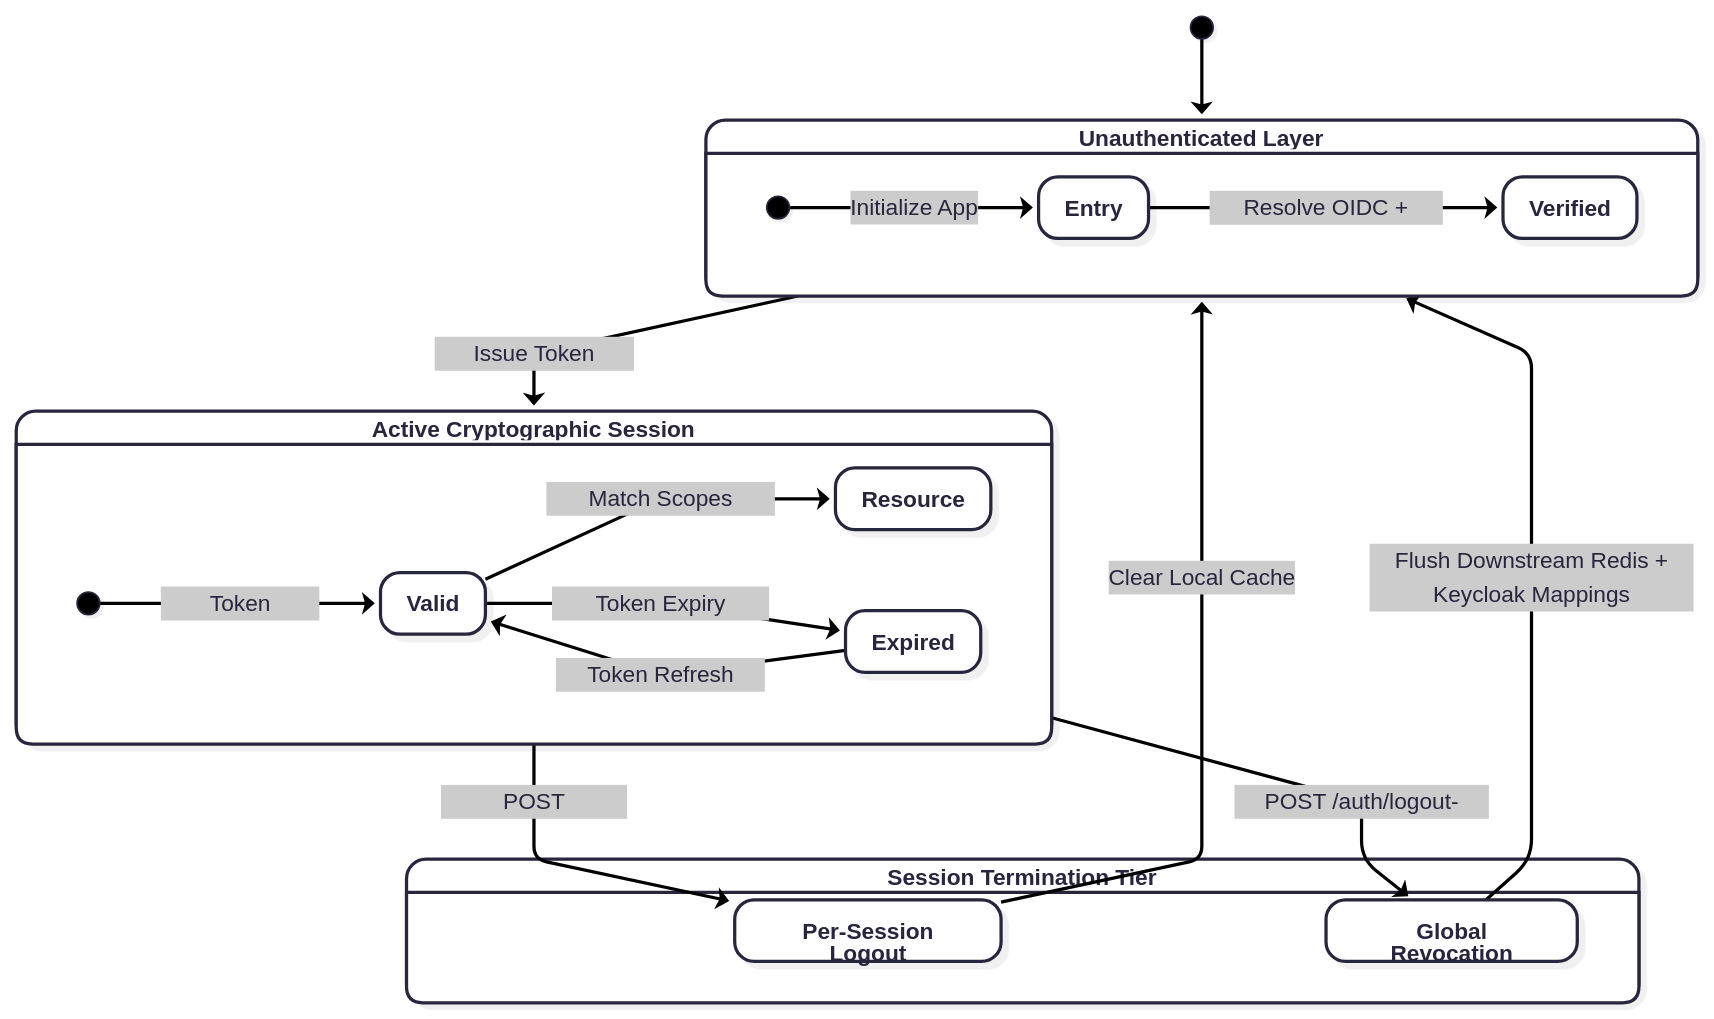
\includegraphics[width=0.7\linewidth]{Security/images/token-flow-overview.png}
    \caption{Token Flow Overview: Unified management of browser and mobile session lifecycles.}
    \label{fig:token-flow-overview}
\end{figure}

\paragraph{Account Management Flow}
Both the browser and mobile applications support Keycloak account-management actions initiated from the practitioner dashboard and patient user profile respectively. 

In the browser's case, a practitioner triggers a password update or TOTP setup from the application, the frontend routes through a backend authentication entry point and includes an \texttt{action} parameter specifying the called account action. 
The backend preserves the intended return destination, forwards the request to Keycloak, and restores the user to the dashboard after the action completes. 
This keeps account-security operations inside the same authenticated flow while avoiding direct client-side exposure of the Keycloak action logic

The mobile application on the other hand handles these same action calls more smoothly through its \texttt{AppAuth} library.


% \subsubsection{Browser Flow }
% The browser is redirected by nginx/\texttt{oauth2-proxy} to Keycloak for login
% (Authorization Code + PKCE) After successful authentication,
% \texttt{oauth2-proxy} maintains the browser session with secure HTTP-only
% cookies and forwards identity headers and access token context to upstream
% services API calls are forwarded to the BFF with \texttt{Authorization: Bearer
%     <token>} added by nginx

% \begin{figure}[H]
%     \centering
%     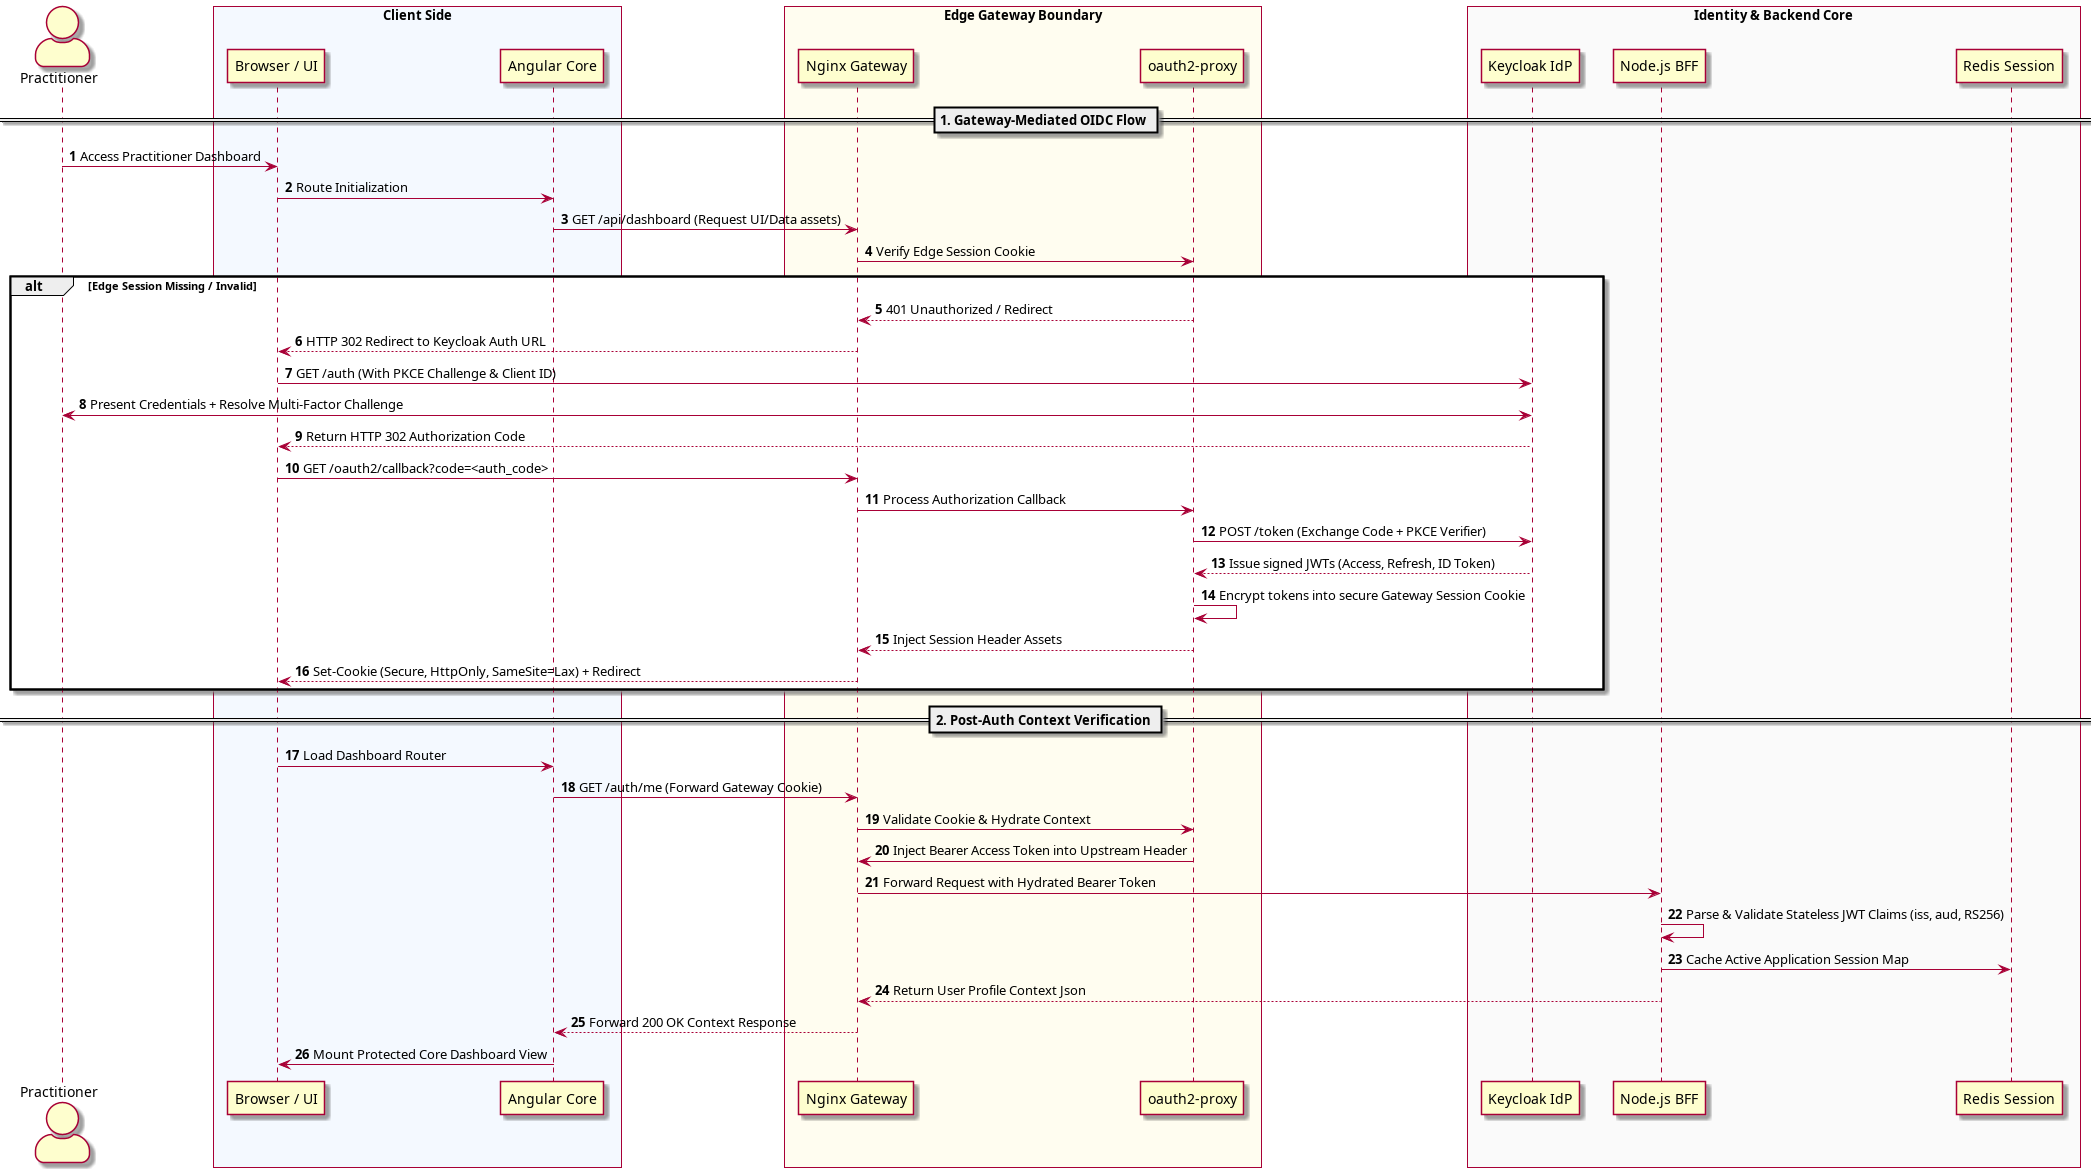
\includegraphics[width=0.9\linewidth]{Security/images/browser-tokens-flow.png}
%     \caption{Browser Token Authentication Flow: User registration, login, and API request handling with session cookies.}
%     \label{fig:browser-tokens-flow}
% \end{figure}

% \paragraph{Browser Email Verification \& MFA}
% Registration is implemented with email verification. Browser-issued accounts
% for practitioners are planned to have an optional MFA addition option

% % \begin{figure}[H]
% %     \centering
% %     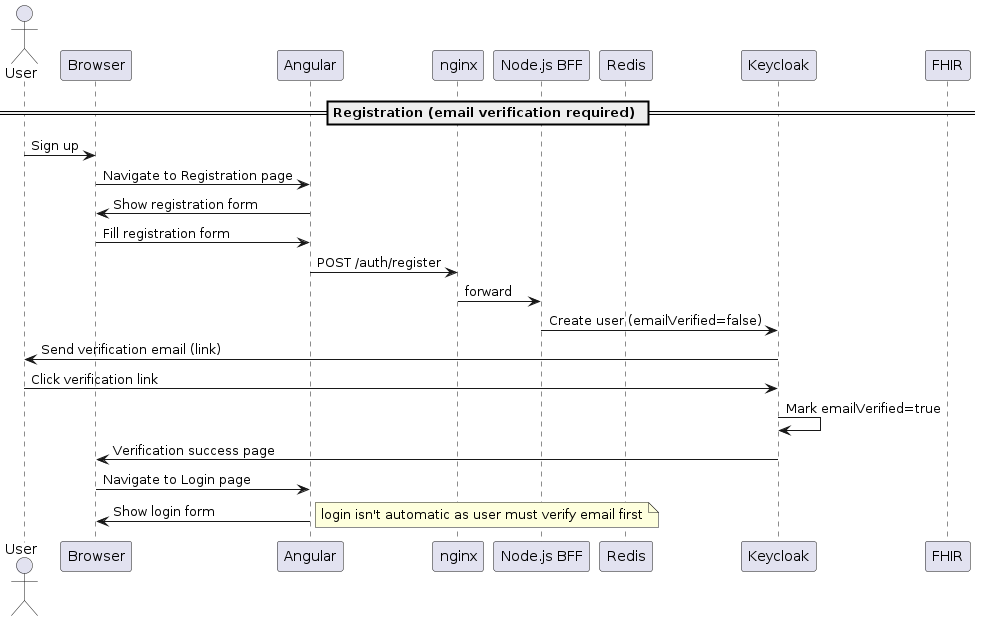
\includegraphics[width=0.8\linewidth]{Security/images/browser-tokens-flow-future.png}
% %     \caption{Planned Browser Flow (Future): Registration with email verification and BFF-mediated credential login, session cookie issuance, and server-side token refresh.}
% %     \label{fig:browser-tokens-flow-future}
% % \end{figure}

% \subsubsection{Mobile Flow}
% For mobile clients, the flow has minor differences from browsers The
% implemented flow uses Authorization Code with PKCE through Keycloak AppAuth
% integration, and stateless access tokens. Tokens are stored in
% platform-specific secure storage (Android Keystore) and sent as
% \texttt{Authorization: Bearer <token>} in API requests. Token refresh is
% client-driven and access tokens are short-lived

% \begin{figure}[H]
%     \centering
%     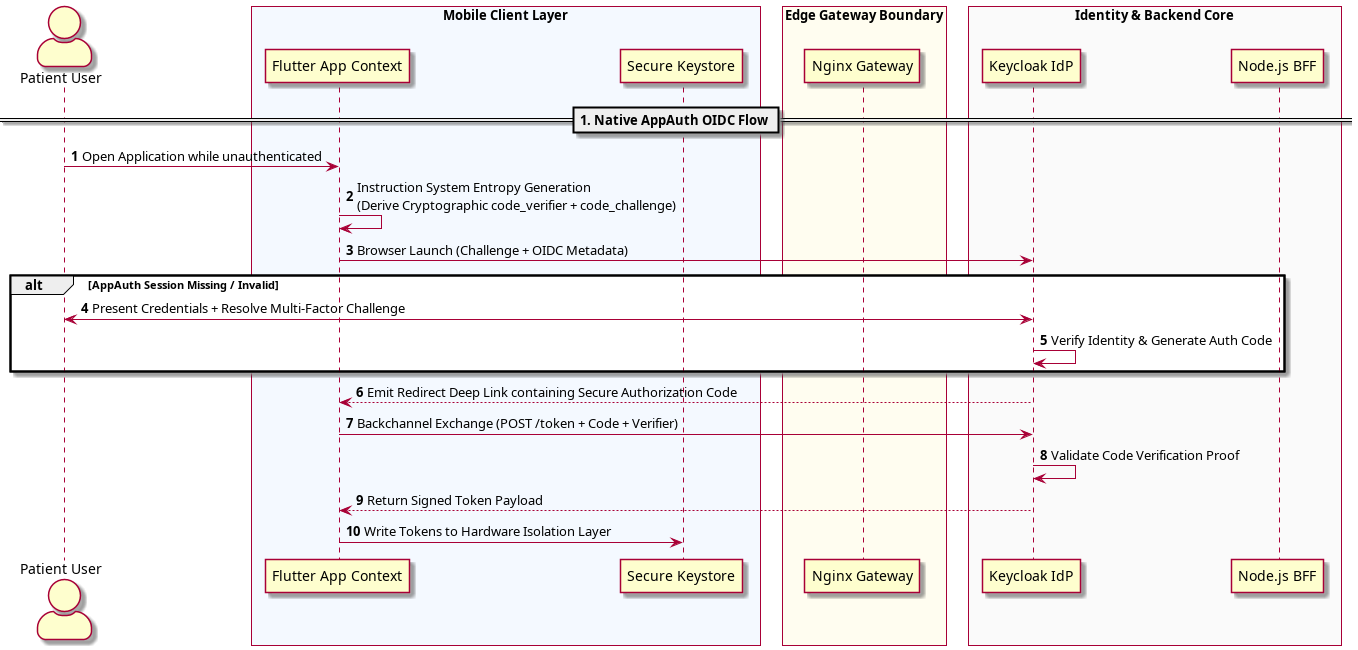
\includegraphics[width=0.8\linewidth]{Security/images/Mobile-tokens-flow.png}
%     \caption{Mobile Authentication Flow: auth code PKCE, secure keystore token storage, and client-driven token refresh.}
%     \label{fig:mobile-tokens-flow}
% \end{figure}

% \subsubsection{Session Middleware (redis), Token Refresh, Token Rotation}
% Express-session with redisStore persists session state, including user
% identity, access token, refresh token, ID token, and their expiration times.
% Browser authentication continuity is handled by the gateway session
% (\texttt{oauth2-proxy} cookies + OIDC flow). The BFF focuses on JWT validation
% for API bearer tokens and session metadata needed for logout-all coordination.
% Session cookies are configured with:
% \begin{itemize}
%     \item \textbf{Secure}: over HTTPS only
%     \item \textbf{HttpOnly}: prevents JavaScript access, mitigating XSS token theft.
%     \item \textbf{SameSite}: set to \texttt{Lax}, blocking CSRF attacks while allowing safe cross-site navigation.
%     \item \textbf{MaxAge}: 1 hour so users must re-authenticate on the browser after inactivity.
% \end{itemize}

% The server is also configured with Helmet, which sets security headers:
% \begin{itemize}
%     \item \textbf{Content-Security-Policy (CSP)}: restricts script sources to \texttt{'self'}, reducing XSS attack surface.
%     \item \textbf{HSTS (Strict-Transport-Security)}: forces HTTPS for 1 year, preventing downgrade attacks.
% \end{itemize}


% \subsection{Session Management \& Revocation}
% The BFF exposes logout endpoints:
% \begin{itemize}
%     \item{Per-session logout}: destroys the current session in redis and revokes refresh tokens at Keycloak's revoke endpoint.
%     \item{Global logout}: removes all user sessions and revokes refresh tokens at Keycloak.
% \end{itemize}

% \begin{figure}[H]
%     \centering
%     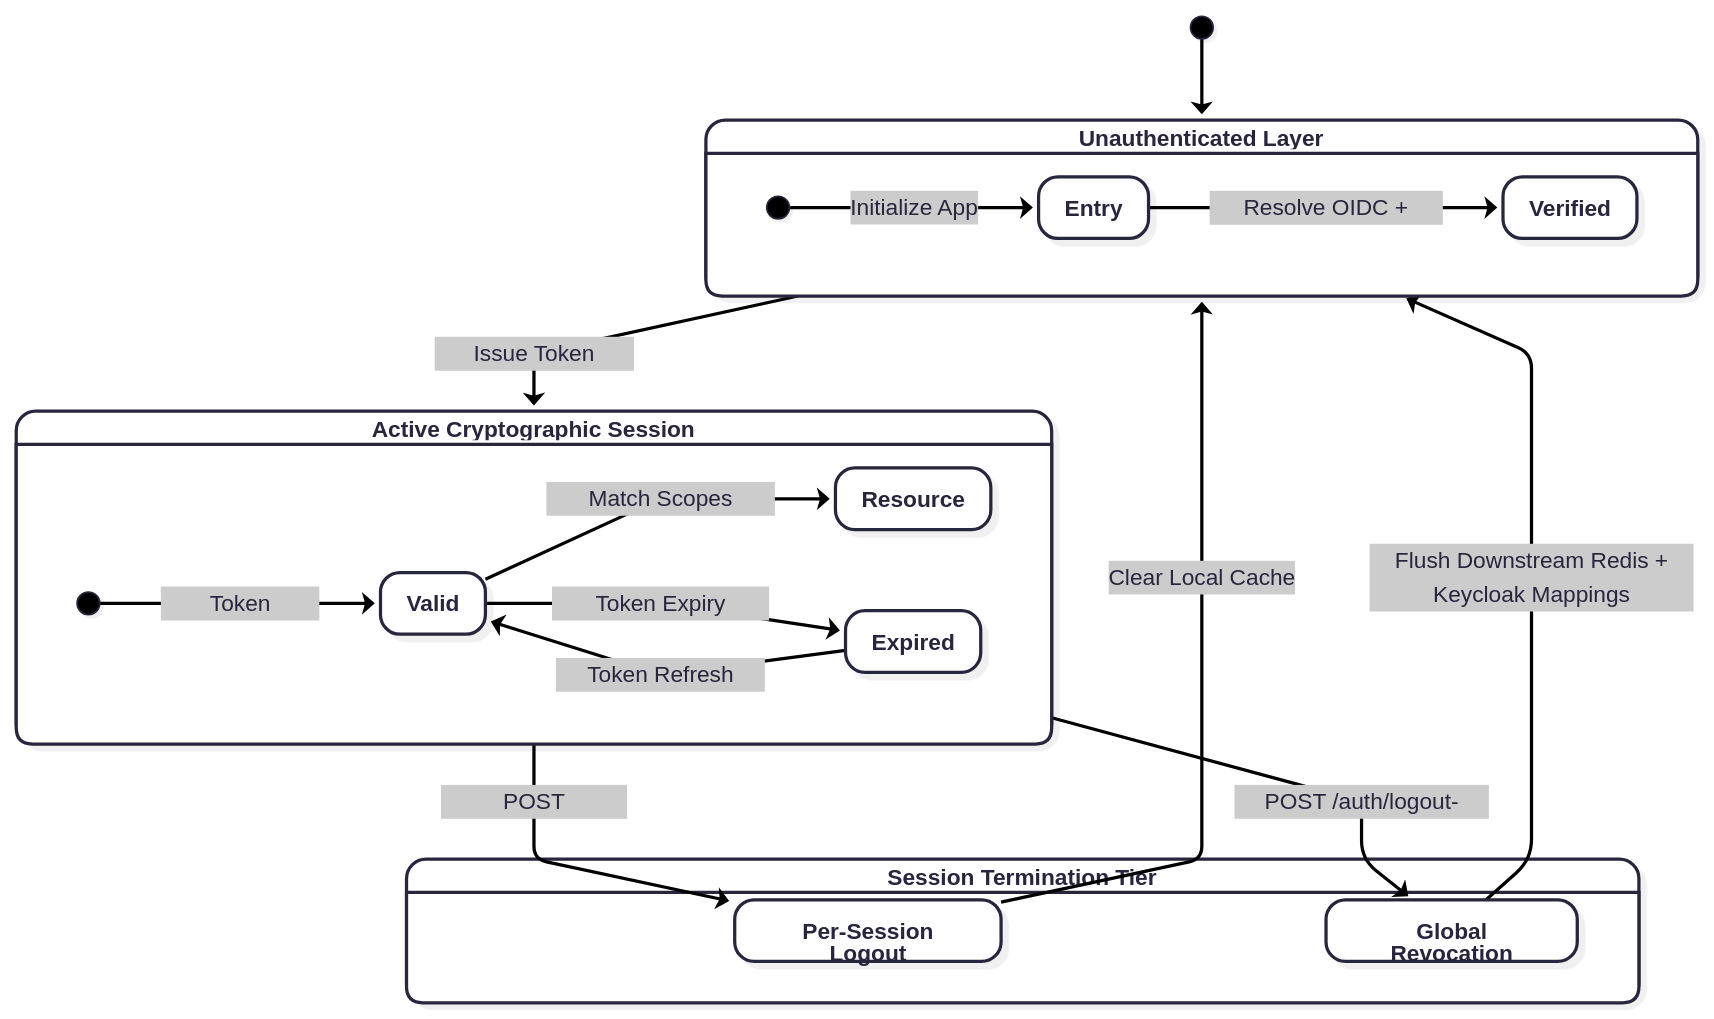
\includegraphics[width=0.7\linewidth]{Security/images/token-flow-overview.png}
%     \caption{Token Flow Overview: Multi-client architecture (browser vs. mobile), session/token management, per-session and global logout patterns.}
%     \label{fig:token-flow-overview}
% \end{figure}

% \paragraph{Session Revocation \& Logout}
% The BFF tracks all active sessions for each user in redis. Per-session logout
% (\texttt{"/logout"}) destroys the current session and revokes current session's
% tokens at Keycloak. Global logout (\texttt{"/logout-all"}) clears all stored
% sessions for the user, rendering all active tokens invalid at the BFF layer.
% The frontend triggers browser sign-out by redirecting to \texttt{/auth/logout},
% which chains \texttt{oauth2-proxy} sign-out and Keycloak logout before
% returning to the application.

% \subsubsection{Session Storage }
% Browser sessions are maintained through oauth2 proxy server. The Proxy server
% saves access/refresh/ID tokens and their expirations. A refresh routine renews
% tokens when they're close to expiry. Backend also stores sessions using
% `express-session' for tracking purposes such as auditing and global logout
% functionality. Session cookies are configured for Secure + HttpOnly, SameSite%using express-session with redisStore

% \subsection{Mobile Authentication Integration}
% Mobile authentication is implemented in the Flutter app using
% `flutter\_appauth' library (Authorization Code + PKCE). The app stores
% \texttt{access}, \texttt{refresh}, and \texttt{id} tokens in secure storage and
% attaches bearer tokens to API requests.

% The app performs client-side refresh when needed and retries protected
% requests. If refresh fails, the app clears session state and redirects to
% login.

% For in-app account security actions, the app invokes Keycloak
% \texttt{kc\_action} flows (e.g., \texttt{UPDATE\_PASSWORD},
% \texttt{CONFIGURE\_TOTP}) and updates local tokens from the returned auth
% response.

% \subsection{oauth2-proxy Integration}
% nginx uses \texttt{auth\_request} to query \texttt{/oauth2/auth}.
% Unauthenticated requests are redirected to \texttt{/oauth2/start}. On success,
% nginx forwards identity headers and access token context to upstream services,
% and injects \texttt{Authorization: Bearer <token>} for protected API routes.

% \subsubsection{Cookie-Based Credentials}
% Session-state endpoints use \texttt{withCredentials: true} \newline
% (\texttt{/auth/session-init}, \texttt{/auth/me}, \texttt{/auth/logout-all}),
% ensuring the Angular HTTP client:
% \begin{itemize}
%     \item Sends session cookies with every request.
%     \item Accepts Set-Cookie headers from the BFF.
% \end{itemize}
% % Without \texttt{withCredentials}, the browser's same-origin policy blocks automatic cookie transmission, breaking session authentication.

% \subsubsection{Angular Frontend Architecture}
% The Angular frontend implements several security layers:

% \paragraph{Route Guards (Authentication Check)}
% Protected routes (dashboard, med-graph/:id) are guarded by \texttt{authGuard},
% a route canActivate function that:
% \begin{itemize}
%     \item Calls AuthService.checkAuthStatus() (a custom function that calls our BFF
%           auth/me endpoint) at route activation.
%     \item Verifies the response's \texttt{authenticated} flag.
%     \item If authenticated, allows route access, otherwise redirects to /login.
% \end{itemize}
% The guard injection follows Angular's functional guard pattern (\texttt{CanActivateFn}), using dependency injection for AuthService and Router.

% \paragraph{Authentication Interceptor (401 Handling)}
% A global HTTP interceptor \\ (\texttt{authInterceptor}) wraps all outbound HTTP
% requests:
% \begin{itemize}
%     \item Catches HTTP responses with status code 401 (Unauthorized).
%     \item Logs a warning message (console.warn) for debugging.
%     \item Redirects to /login, clearing the current route and forcing re-authentication.
%     \item Re-throws the error after routing, allowing components to handle error states.
% \end{itemize}
% This provides automatic session expiry handling: if the backend session expires or tokens are revoked, the first 401 response triggers a redirect, preventing continued access to stale sessions.


% \subsubsection{Mobile App (Flutter) Security Architecture}
% The implemented mobile architecture includes:
% \begin{itemize}
%     \item \textbf{Secure Token Storage}:
%           \begin{itemize}
%               \item Android: Keystore system.
%           \end{itemize}
%     \item \textbf{Bearer Token Auth}: Each HTTP request includes \texttt{Authorization: Bearer <access\_token>} header.
%     \item \textbf{Authorization Code + PKCE}: Implemented through Keycloak AppAuth.
%     \item \textbf{Token Refresh Logic}: Mobile app implements its own refresh routine (unlike browser, where the proxy server handles refresh):
%           \begin{itemize}
%               \item On 401 response, perform refresh grant.
%               \item Retry the original request with the new token.
%               \item If refresh fails, clear tokens and redirect to login.
%           \end{itemize}
%     \item \textbf{Account Security Actions}: In-app flows for \texttt{UPDATE\_PASSWORD} and \texttt{CONFIGURE\_TOTP} %are executed using Keycloak \texttt{kc\_action}.
%     \item \textbf{Certificate Pinning} (future work): pin the BFF's TLS cert in the mobile app to prevent MITM attacks by rogue CAs.
%           % \item \textbf{App Transport Security (ATS)}: Enforce HTTPS only and require strong TLS versions (1.2+) by default.
% \end{itemize}

% % \paragraph{Third-Party Dependencies}

% % Future work: Pin exact versions in package.json and regularly audit for
% % vulnerabilities % (using \texttt{npm audit}).



